\section{Datasets}\label{dataset}
In order to create metamorphic properties that can be used by multiple image datasets and are not data-dependent, we tested our metamorphic properties on three different datasets. We choose the following three datasets, but the experiment can be easily replicated on other image datasets.

\subsection{MNIST Dataset}
% The MNIST database of handwritten digits maintained by Yann LeCun \cite{MNIST} has a training set of 55,000 examples and a test set of 10,000 examples. It is a subset of a larger set available from NIST. The digits have been size-normalized and centered in a fixed-size image. It is an excellent database for people who want to try learning techniques and pattern recognition methods on real-world data while spending minimal efforts on preprocessing and formatting. The MNIST database was constructed from NIST's Special Database 3 and Special Database 1, which contain binary images of handwritten digits. The original black and white (bi-level) images from NIST were size normalized to fit in a 20x20 pixel box while preserving their aspect ratio. The images were centered in a 28x28 image by computing the center of mass of the pixels, and translating the image so as to position this point at the center of the 28x28 field.
Yann LeCun maintains one of the most popular databases for machine learning algorithms. The MNIST database is a collection of $55,000$ training images and $10,000$ test images \cite{MNIST}.  The MNIST dataset is a subset of a larger NIST dataset - Special Database 3 and Special Database 1. The images in the dataset are handwritten digits samples between $[0,9]$, which are size-normalized and centered in a 28x28 pixel image. The original images were size normalized into a 20x20 pixel box while preserving their aspect ratio. The images were converted to 28x28 pixel by first calculating their center of mass and then translating the images such that the center of mass is on the center of the 28x28 field. The following figuire shows a sample set of MNIST data.
\begin{figure}[htb!]
\centering
    \centering
    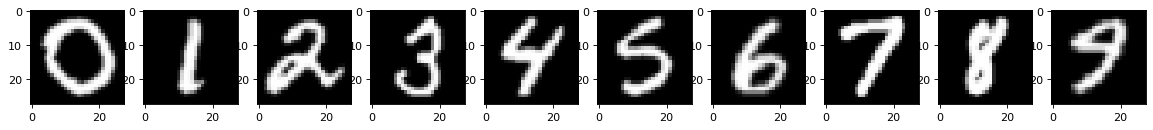
\includegraphics[width=\linewidth]{images/digit.png}
    \caption{Sample MNIST dataset}
    \label{fig:EMNIST MNIST dataset}
\end{figure}
      
\subsection{EMNIST Dataset}
% The EMNIST dataset is a set of handwritten character digits derived from the NIST Special Database 19
% and converted to a 28x28 pixel image format. 
The EMNIST dataset has the same shape as MNIST dataset. They are 28x28 pixels of handwritten characters that are derived from the "NIST Special Database 19". There are six different splits provided in this dataset. The splits are organized by class, by balance, by type, etc. Some splits are unbalanced and contain an uneven number of examples for classes. The EMNIST-Digit and EMNIST-MNIST datasets are directly compatible with the original MNIST dataset. For this study, we choose "EMNIST Letters" split, which has $119,800$ characters in 26 balanced classes where each class has the same number of samples. The characters are in uppercase and lowercase, which have have been merged into one 26-class set.
The figure \ref{fig:emnist-letter} shows a sample image of the EMNIST-Letter dataset.

\begin{figure}[htb!]
        \centering
    
            \centering
            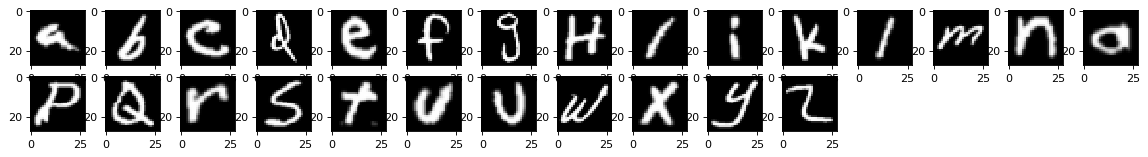
\includegraphics[width=\linewidth]{images/letter.png}
            \caption{Sample EMNIST-Letter dataset}
            \label{fig:EMNIST MNIST dataset}
        \label{fig:emnist-letter}
    \end{figure}
    \FloatBarrier

    
\subsection{Fashion MNIST Dataset}
A dataset of Zalando's article images which consist of a set of $55,000$ training examples and $10,000$ test examples. The dataset is commonly referred to as the Fashion-MNIST dataset. Every data point in the dataset is a grayscale image of size 28x28. The labels in the dataset have a value between $[0, 9]$. Table \ref{tbl:MNIST-Fashion} shows a sample of the dataset.

\begin{table}[ht]
\centering
\begin{tabular}{|c|c|}
\hline
\textbf{Label} & \textbf{Description} \\ \hline
0  &   T-shirt/top \\ \hline
1  &   Trouser \\ \hline
2   &	Pullover \\ \hline
3   &	Dress \\ \hline
4   &	Coat \\ \hline
5   &	Sandal \\ \hline
6   &	Shirt \\ \hline
7   &	Sneaker \\ \hline
8   &	Bag \\ \hline
9   &	Ankle boot \\ \hline
\end{tabular}
\caption{Data file format.}
\label{tbl:MNIST-Fashion}
\end{table}

\begin{figure}[htb!]
        \centering
        \begin{subfigure}[b]{\textwidth}
            \centering
            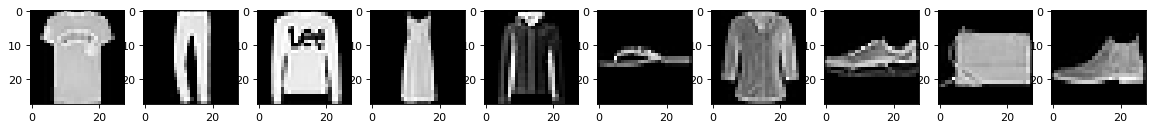
\includegraphics[width=\linewidth]{images/fashion.png}
            \caption{Sample Fashion-MNIST dataset}
            \label{fig:EMNIST MNIST dataset}
        \end{subfigure}%
        \label{fig:Rotate-misclassifications}
    \end{figure}
    \FloatBarrier
    
\subsection{Format of Dataset}
Each dataset we selected has the same file structure. The data is stored across four files. The "train-images-idx3-ubyte" and "train-labels-idx1-ubyte" files contain the training images and labels, respectively. The "t10k-images-idx3-ubyte" and "t10k-labels-idx1-ubyte" files contain the test images and labels. The labels for the MNIST and Fashion-MNIST are between $[0, 9]$, while the labels for EMNIST-LETTER are between $[1, 26]$. The integers in the files are stored in MSB first format (high endian).

The format of training and test files are described in the following table.
\begin{table}[H]
\centering
\begin{tabular}{|c|c|c|c|}
\hline
\textbf{offset} & \textbf{type}    &      \textbf{value}    &      \textbf{description} \\
\hline
0000  &   32 bit integer & 0x00000801(2049) & magic number (MSB first) \\
\hline
0004  &   32 bit integer & 60000       &     number of items \\
\hline
0008  &   unsigned byte  & ??          &     label \\
\hline
0009  &   unsigned byte  & ??          &     label \\
\hline
\multicolumn{4}{|c|}{\textbf{........}} \\
\hline
xxxx  &   unsigned byte  & ??          &     label \\
\hline
\multicolumn{4}{|c|}{\textbf{The label values are 0 to 9.}} \\
\hline
\end{tabular}
\caption{Training data file format.}
\label{tbl:training-file-format}
\end{table}

\begin{table}[H]
\centering
\begin{tabular}{|c|c|c|c|}
\hline
\textbf{offset} & \textbf{type}    &      \textbf{value}    &      \textbf{description} \\
\hline
0000  &   32 bit integer & 0x00000803(2051) & magic number (MSB first) \\
\hline
0004  &   32 bit integer & 60000       &     number of images \\
\hline
0008  &   unsigned byte  & 28          &     number of rows  \\
\hline
0012  &   unsigned byte  & 28          &     number of columns \\
\hline
0016  &   unsigned byte  & ??          &     pixel \\
\hline
0017  &   unsigned byte  & ??          &     pixel \\
\hline
\multicolumn{4}{|c|}{\textbf{........}} \\
\hline
xxxx  &   unsigned byte  & ??          &     pixel \\
\hline
\multicolumn{4}{|c|}{\textbf{
\shortstack{Pixels are organized row-wise. Pixel values are 0 to 255. \\ 0 means background (white), 255 means foreground (black).}}} \\
\hline
\end{tabular}
\caption{Test data file format.}
\label{tbl:test-file-format}
\end{table}